% !TEX program = xelatex

\documentclass[10pt, compress,notheorems]{beamer}

\usetheme{m}

\usepackage{booktabs}
\usepackage[scale=2]{ccicons}
\usepackage{minted}
\usepackage{amsmath}
\usepackage{bm}
\usepackage{hyperref}
\usepackage{url}
\usepackage{graphicx}
\usepackage{multirow}
\usepackage{multicol}
\usepackage{amsfonts}
\usepackage{pgf,tikz}
\usepackage{tgpagella}
\usepackage{centernot}
\usepackage{caption}

\usepackage{graphicx}

\usepgfplotslibrary{dateplot}

\usemintedstyle{trac}

\title[Composite Indicators]{Pathway 2: Developing Composite Indicators}
\subtitle{}
\date{}
\author{
    \href{mailto:christopher.gandrud@city.ac.uk}{Christopher Gandrud}
}
\institute{SG1022, City University London}

\begin{document}

\maketitle

\section{Aims}

\frame{
    \frametitle{Aims}

    \begin{itemize}
        \item What are composite indicators and who uses them?

        \item Defining the construct and what can be observed.

        \item Making Composite Indicators

            \begin{itemize}
                \item What data to include?

                \item How to normalise the variables?

                \item How to weight the variables?

                \item Assessing validity (introduction)
            \end{itemize}

        \item Pros, cons, and pitfalls

        \item Survey examples
    \end{itemize}

}

\section{What are Composite Indicators}

\frame{
    \frametitle{Variables}

    Last semester, we learned about {\large{concepts}} and {\large{variables}}.

    \begin{itemize}
        \item \emph{Concept}: A phenomenon (e.g. poverty, democracy, human development, trust in institutions) we are interested in studying.

        \vspace{0.5cm}

        \item \emph{Variable}: Observable characteristic of a unit (e.g. person, city, country) that operationalises the concept.
    \end{itemize}

}

\frame{

    \begin{center}
        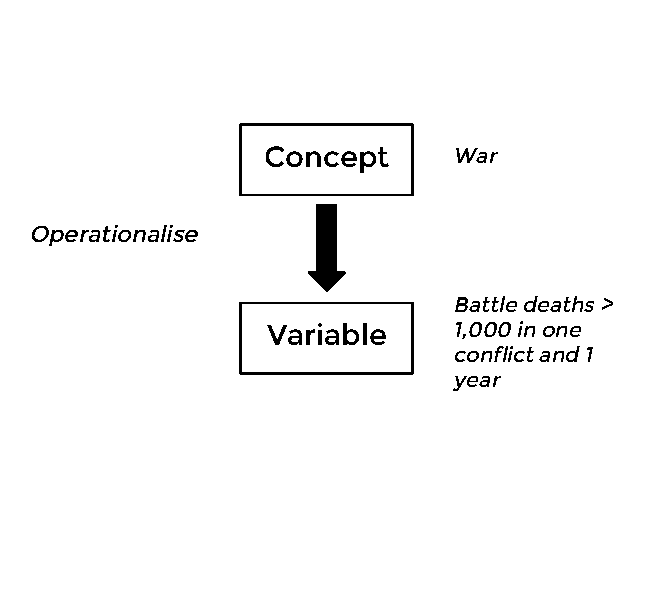
\includegraphics[scale=0.7]{figures/concept_variable.pdf}
    \end{center}
}

\frame{
    \frametitle{When one variable is not enough}

    Frequently in social science we are interested in {\large{complex concepts that cannot be operationalised with one variable}}.

    \vspace{0.5cm}

    Instead, they likely involve {\large{some combination of variables}}.

}

\frame{
    \frametitle{What is it?}

    \begin{center}
        For example, what is democracy?
    \end{center}

}

\frame{
    \frametitle{What is democracy?}

    {\large{Conceptualisation}}: Dahl (1971) argued that democracy has two core attributes:

    \begin{itemize}

        \item \emph{contestation}: competitive elections to choose leaders,

        \item \emph{participation}: inclusive rules for and rates of participation.

    \end{itemize}

    \vspace{0.5cm}

    Note: not just elections/no elections or universal suffrage/limited suffrage. So \ldots

}

\frame{

    \begin{center}
        \ldots we need a {\large{composite indicator}} to operationalise Dahl's conceptualisation of democracy.
    \end{center}

}

\frame{
    \frametitle{Creating the Polity IV Democracy Index}

    \begin{center}
        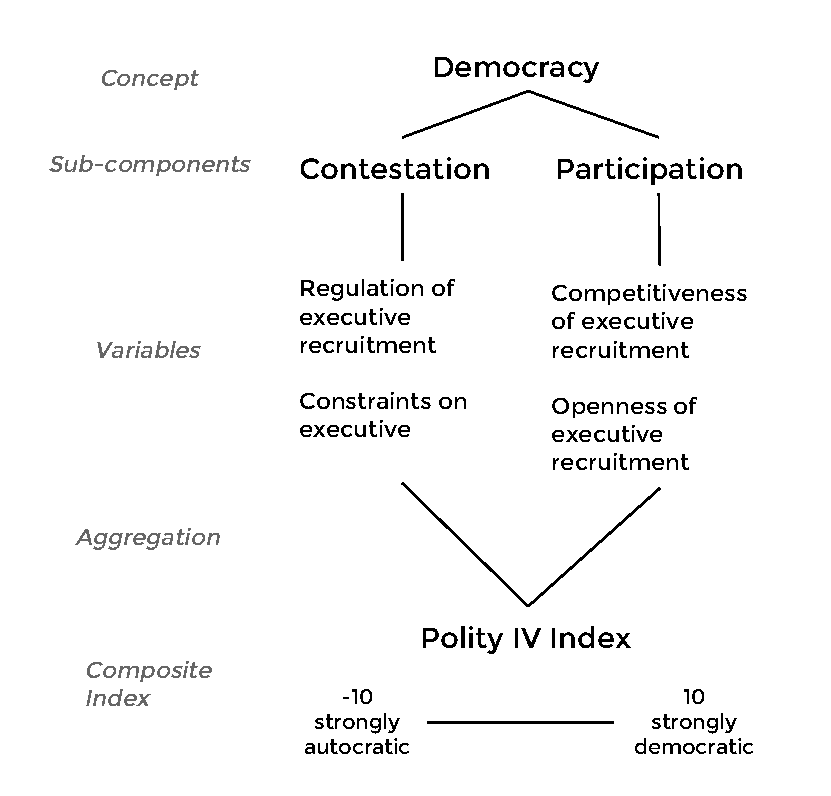
\includegraphics[scale=0.55]{figures/polity_construction.pdf}
    \end{center}

}

\frame{
    \frametitle{Pakistan Polity IV Score}

    \begin{center}
        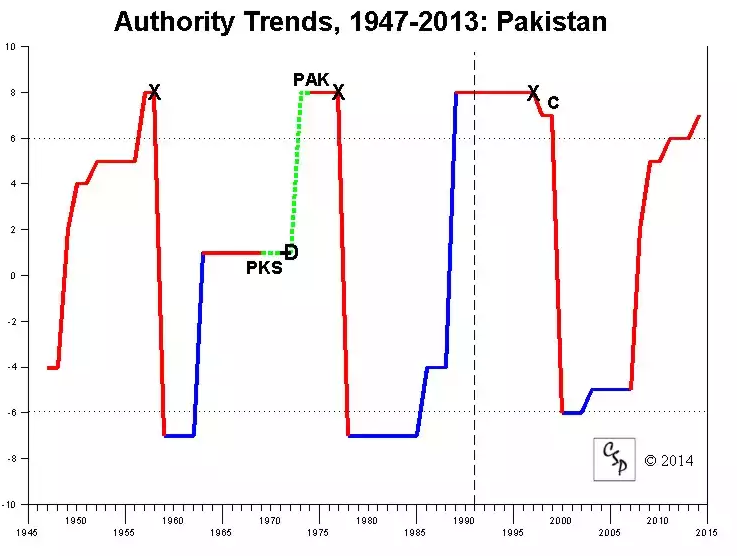
\includegraphics[scale=0.37]{figures/pakistan_polity.png}
    \end{center}

}

\frame{
    \frametitle{Why care?}

    \begin{center}
        {\large{Why should we care about measuring concepts well?}}
    \end{center}
}

\frame{
    \frametitle{Why care?}

    \begin{center}
        If we don't have good measures of our concepts, {\large{we can't know how one thing effects another (relationships \emph{between} concepts) and how to improve the social world}}.
    \end{center}
}

\frame{
    \frametitle{Composite indicators and policy-making}

    Composite indicators are a popular tool used by governments, international organisations, NGOs, and public policy advocacy groups.

}

\frame{
    \frametitle{IMF Fiscal Transparency (GFS) Index}

    \begin{center}
        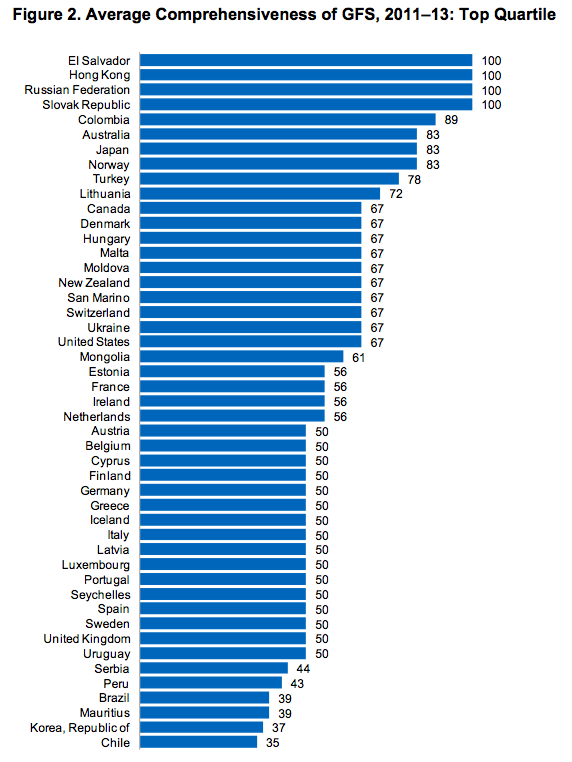
\includegraphics[scale=0.25]{figures/gfs.png}
    \end{center}

    {\tiny{Wang et al. (2015, 10)}}

}

\frame{
    \frametitle{University rankings}

    \begin{center}
        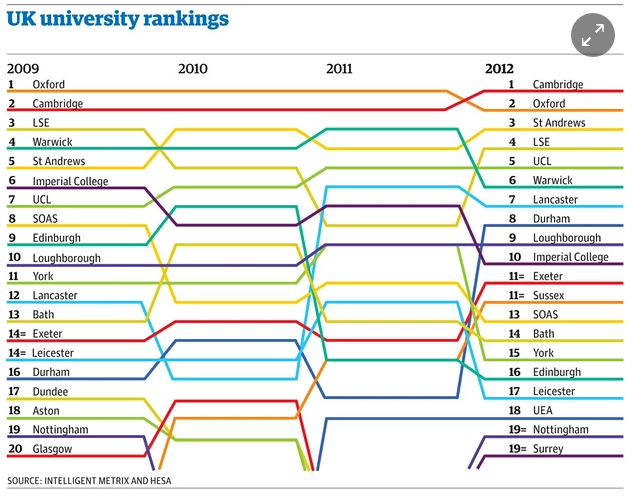
\includegraphics[scale=0.35]{figures/university_ranking.png}
    \end{center}

    {\tiny{(http://www.theguardian.com/news/datablog/2011/may/17/university-guide-2012-data-guardian)}}

}

\frame{
    \frametitle{Global Financial Centres Index (2015)}

    \begin{center}
        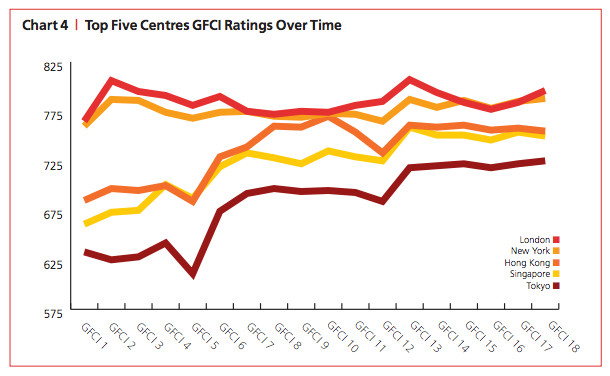
\includegraphics[scale=0.4]{figures/gfci_ranking.png}
    \end{center}

    {\tiny{Z/Yen Group (2015, 8)}}

}

\frame{
    \frametitle{Impacts our understanding of the world and policymaking}

    \begin{center}
        
\includegraphics[scale=0.4]{figures/gfc_headline.png}
    \end{center}

    {\tiny{Financial Times (1 Oct 2014)}}

}

\section{Steps to Creating Composite Indicators}

\frame{
    \frametitle{Steps for Building Composite Indicators}

    \begin{enumerate}
        \item Theoretical framework

        \item Data selection

        \item Address missing data

        \item Multivariate analysis (note: we don't really cover this in this course)

        \item Normalisation

        \item Weighting and aggregation

        \item Validation

    \end{enumerate}

    {\tiny{Modified from OECD (2008, 20-21)}}

}

\frame{

    \begin{center}
        All of these steps should be {\LARGE{clearly documented in detail}}.
    \end{center}

}

\section{Theoretical Framework}

\frame{
    \frametitle{Conceptualisation}

    \begin{center}
        ``What is {\LARGE{badly defined}} is likely to be {\LARGE{badly measured}}.'' {\tiny{(OECD 2008, 22)}}
    \end{center}

}

\frame{
    \frametitle{Defining the concept}

    {\large{Concept definitions should}}:

    \begin{itemize}

        \item be clear and parsimonious,

        \item refer to a theoretical framework,

        \item select a relevant unit of analysis,

        \item link various sub-grous and the underlying indicator.

    \end{itemize}

}

\frame{
    \frametitle{Sub-components}

    {\large{Sub-components}}:

    \begin{itemize}

        \item should be \emph{statistically independent} of each other (want as few components as possible, don't want to double up),

        \item existing \emph{linkages} between them should be \emph{described theoretically and empirically} as much as possible.

    \end{itemize}

}

\frame{
    \frametitle{Conceptualising democracy}

    \begin{center}
        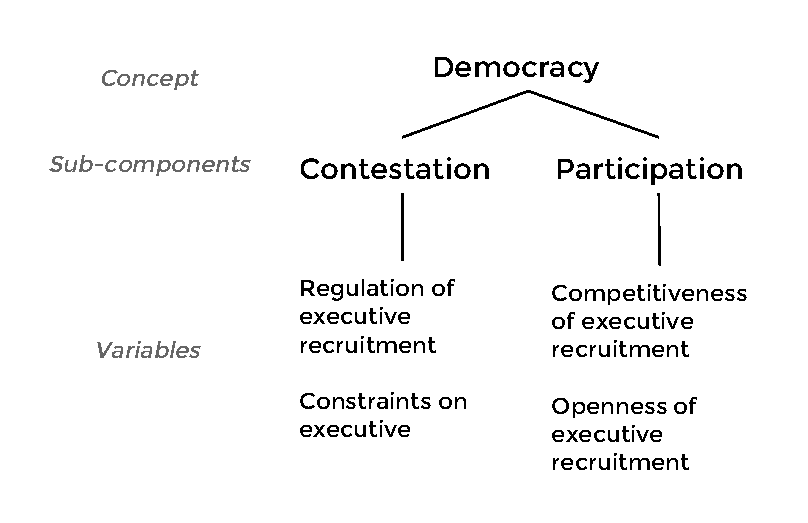
\includegraphics[scale=0.55]{figures/democracy_conceptualisation.pdf}
    \end{center}

}


\section{Data Selection}

\frame{
    \frametitle{Data selection}

    A composite indicator is {\large{only as good as its parts}}.

    \vspace{0.5cm}

    Data on the indicators' component should be selected based on at least their:

    \begin{itemize}

        \item relevance to the theoretical framework,

        \item analytical soundness,

        \item timeliness,

        \item accessibility.

    \end{itemize}

}

\frame{
    \frametitle{Gathering, cleaning, merging}

    \begin{center}
        Gathering, cleaning, and merging the component variables is {\large{not trivial}}.

        \vspace{1cm}

        Has important {\large{substantive implications}} (e.g. error can bias your indicators) and can be {\large{time consuming}}.

        \vspace{1cm}

        So, needs to be well documented and {\large{reproducible}}.
    \end{center}

}

\section{Missing data}

\frame{
    \frametitle{Missing values}

    \begin{center}
        To aggregate your components into a composite indicator you need a {\large{complete data set}}, with {\large{no missing values}}.

        \vspace{0.5cm}

        For example, imagine we are going to make a component indicator with \textt{variable\_1}, \textt{variable\_2}, and \textt{variable\_3}. A complete data set would look like:

    \begin{table}
        \begin{tabular}{l c c c}
            country & variable\_1 & variable\_2 & variable\_3 \\
            \hline
            Algeria & 1 & 10034 & 0 \\
            Cambodia & 0 & 30020 & 0 \\
            Zambia & 0 & 50302 & 1 \\
            \hline
        \end{tabular}
    \end{table}

    \end{center}

}

\frame{

    \frametitle{Missing values}

    \begin{center}
        However, we often (especially when working with country-level data) have missing data on at least some of our variables.

        \vspace{0.5cm}

        For example:

        \begin{table}
            \begin{tabular}{l c c c}
                country & variable\_1 & variable\_2 & variable\_3 \\
                \hline
                Algeria & NA & 10034 & 0 \\
                Cambodia & 0 & 30020 & 0 \\
                Zambia & 0 & NA & 1 \\
                \hline
            \end{tabular}
        \end{table}

    \end{center}

Note: NA in R means missing value.

}

\frame{

    \frametitle{Missing values}

    \begin{center}
        You should always assess {\large{how much}} missing data you have and {\large{consider why}} the data is missing.

    \end{center}

}

\frame{
    \frametitle{Why missing}

    Data can be:

    \begin{itemize}
        \item \emph{Missing at random}: why the variable value is missing has nothing to do with the variable--random.

        \item \emph{Not missing at random}: the variable value is missing because of some reason related to the variable.

        \begin{itemize}
            \item E.g.: Low income countries don't have the money to pay for enough staff to gather GDP data.
        \end{itemize}

    \end{itemize}

}

\frame{
    \frametitle{Why missing}

    Not missing at random is complex to deal with and requires explicit modeling of the missing process.

    \vspace{1cm}

    We do not cover this modeling process in this course.

    \vspace{1cm}

    However, if you suspect your data is not missing at random, you should discuss this including the reasons why you believe this.

}

\frame{
    \frametitle{Addressing missing data}

    If you have missing data, to get complete cases you can:

    \begin{itemize}
        \item drop incomplete cases,

        \item single impute data (e.g. replacing the missing value with the variable's mean/median/mode),

        \item multiple impute data (not covered in this course).
    \end{itemize}

}

\section{Analysis of the component structure}

\frame{
    \frametitle{Underlying structure}

    \begin{center}
        ``Analysing the {\large{underlying structure}} of the data is still an {\large{art}}.'' {\tiny{(OECD 2008, 25)}}

        \vspace{1cm}

        Understanding the underlying structure is important for informing weighting and aggregation decisions.

        Note: important multivariate analysis tools--e.g. principal component analysis, cluster analysis--are {\large{beyond the scope of this class}}.
    \end{center}

}

\frame{
    \frametitle{Simple correlation analysis}

    A simple way to examine the relationships between your sub-components is to create a {\large{correlation matrix}}.

    \vspace{0.5cm}

    {\large{Correlation}}: a mutual relationship between two variables.

    \vspace{0.5cm}

    {\large{Correlation coefficient}}: a number ranging from -1 to 1 calculated to represent the linear correlation between two variables. Usually denoted $r$.
}

\frame{

    \begin{center}
        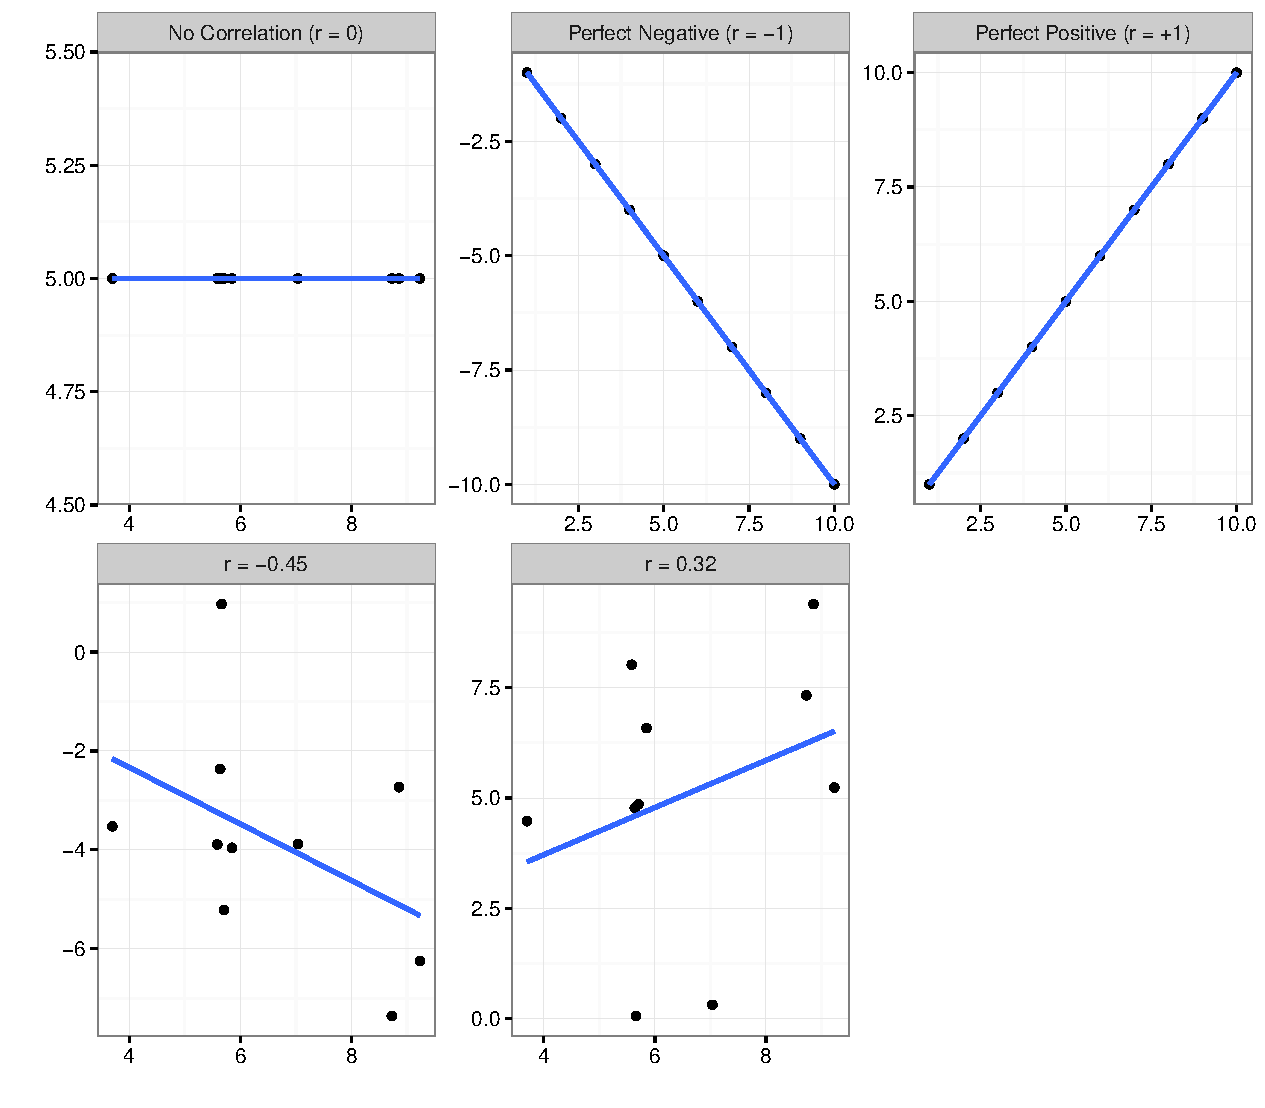
\includegraphics[scale=0.5]{figures/corr_plot_example.pdf}
    \end{center}

}

\frame{
    \frametitle{Correlation matrix}

    \begin{center}
        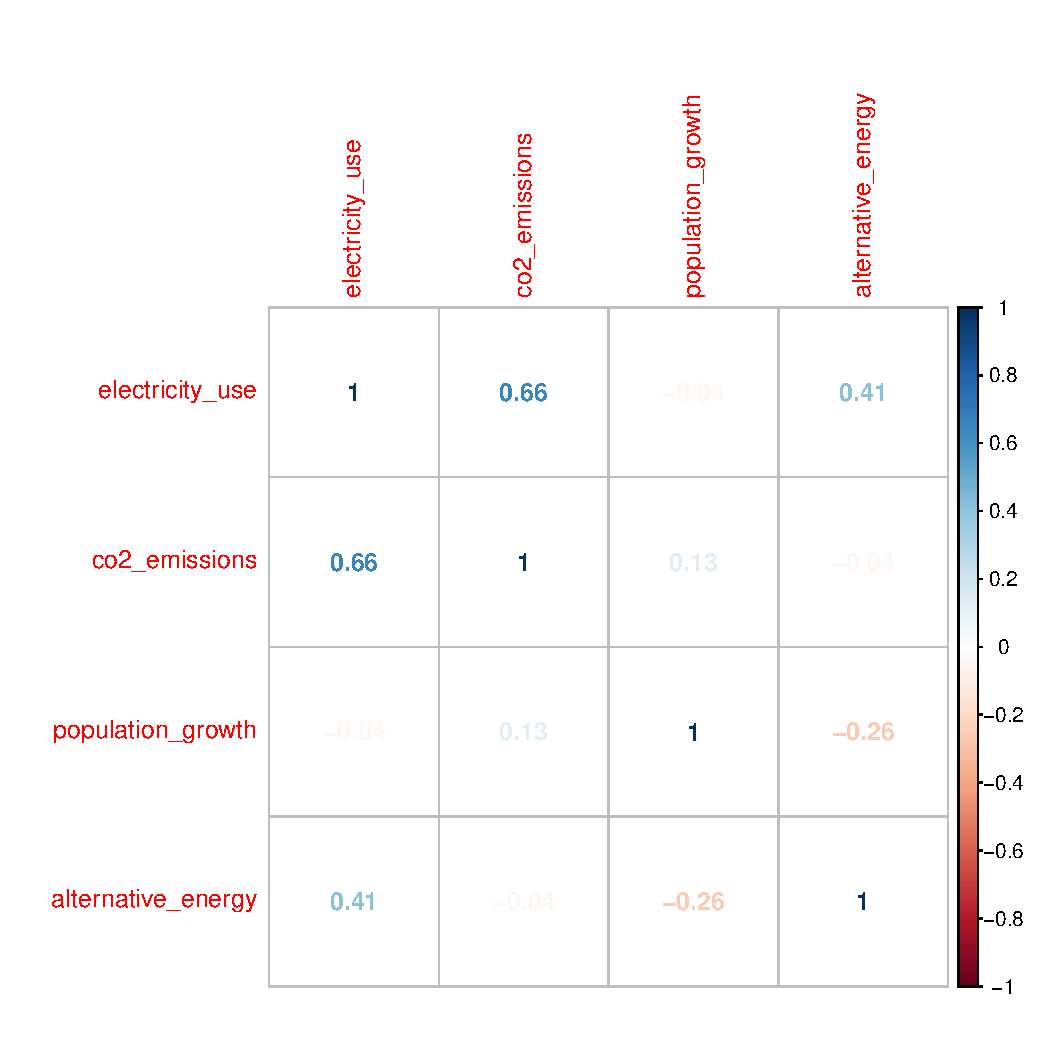
\includegraphics[scale=0.45]{figures/energy_corr.pdf}
    \end{center}

}

\section{Normalise variables}

\frame{
    \frametitle{On a level playing field}

    Observable variables are often on {\large{\textbf{different scales}}} as they can have {\large{different measurement units}}.

    \vspace{0.5cm}

    For example, \emph{life expectancy at birth} is in years ranging from 0 to $>100$ and \emph{GNI per capita} is in US dollars starting from $>300$.

    \vspace{0.5cm}

    Obviously, adding these two variables together would {\large{\textbf{weight GNI more than life expectancy}}}.
}

\frame{
    \frametitle{Some notation}

    Some notation:

    \begin{itemzie}
        \item $x_{i,t}$: Observed variable value for unit $i$ (e.g. country) at time $t$ (e.g. year)

        \item $I_{i,t}$ Normalised value of the variable value for unit $i$ at time $t$
    \end{itemize}

}

\section{Weighting and Aggregation}

\frame{
    \frametitle{Why weight?}

    Once you have your normalised variables ($I_{c,t}$), then you need to consider how to {\large{\textbf{combine}}} them.

    Things to consider:

    \begin{itemize}
        \item {\large{\textbf{Weighting}}}: how important are each individual variables to the composite?

        \item What {\large{\textbf{scale}}} do you want the indicator to be on?
    \end{itemize}
}

\frame{

    \begin{center}
        ``No uniformly agreed methodology exists to weight individual indicators before aggregating them into a composite indicator.''

        \vspace{1cm}

        But generally, ``what matters more \ldots weighs more.''

        {\tiny{https://composite-indicators.jrc.ec.europa.eu/?q=content/step-6-weighting}}
    \end{center}

}

\frame{
    \frametitle{Equal weighting}

    If you simply {\large{\textbf{add all of the variables}}} together, you are implicitly assuming that they have an {\large{\textbf{equal weight}}} of {\large{\textbf{1}}}.

    \begin{equation}
        CI_{c,t} = \sum I_{c,t}*1
    \end{equation}

    Sometimes this makes sense: e.g. economic activity is often measured in the same currency.

}

\frame{
    \frametitle{Unequal weighting}


}

\frame{
    \frametitle{Threshold aggregation}

    Sometimes the concept we are measuring might be discrete. E.g. you are in a financial crisis or not in a financial crisis.

    \vspace{0.5cm}

    So, you might set a {\LARGE{threshold}}, a point past which a unit goes from having the characteristic to not having the characteristics.

}

\frame{
    \frametitle{Threshold example}

    Laeven and Valencia (2013) determine a country has crossed a {\large{financial crisis threshold}} if:

    \begin{itemize}
        \item There is `signficant distress' in a country's financial system.

            \begin{center}
                \emph{and}
            \end{center}

        \item At least three of six policy responses are used (e.g. bank holidays, bank nationalisations).
    \end{itemize}
}

\frame{
    \frametitle{Laeven \& Valencia Banking Crises (1970-2011)}

    \begin{center}
        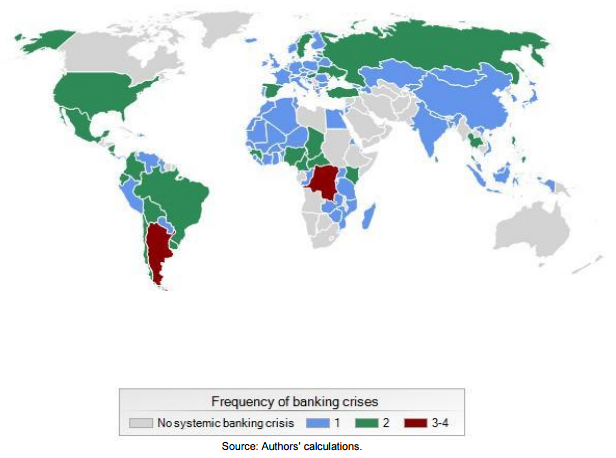
\includegraphics[scale=0.45]{figures/banking_crisis_map.png}
    \end{center}

}

\section{What are we measuring?}

\frame{
    \frametitle{Validity}

    Once you have a composite indicator, your work is {\large{\textbf{far from done}}}.

    \vspace{0.5cm}

    You need to conduct numerous tests to determine if your indicator is a {\large{\textbf{valid}}} measure of the concept you are tying to measure.

}

\frame{
    \frametitle{Transparency}

    There is likely {\LARGE{no perfect composite indicator}} for any given concept.

    \vspace{0.5cm}

    {\LARGE{Transparency}}--conceptualisation, data gathering/cleaning, construction, validation--is crucial for others to be able to {\large{understand}} and {\large{evaluate}} your indicators.
}

\section{Pros and Cons}

\frame{
    \frametitle{Uncertainty}

    {\large{\textbf{However}}}, we need to remember that our indicators are {\LARGE{\textbf{estimates}}} of what we want to measure.

    \vspace{0.5cm}

    We are {\LARGE{\textbf{uncertain}}} about how well our indicators capture reality.

    \vspace{0.5cm}

    Uncertainty can be {\large{caused}} by at least:

    \begin{itemize}

        \item Error in our construct (i.e. including or omitting important variables)

        \item Measurement error in our raw data $x_{c,t}$

        \item Error in our weighting.

    \end{itemize}

}

\frame{
    \frametitle{Ranking}

    Composite indicators are popularly used to {\large{\textbf{rank units}}} (e.g. cities, countries).

    \vspace{0.5cm}

    However, this can be {\LARGE{highly misleading}}.
}

\frame{
    \frametitle{Ranking Example}

    For example, Copelovitch, Gandrud, and Hallerberg (2015) created a measure of financial supervisory transparency.

    \begin{table}
        \caption{Financial Regulatory Transparency Index Ranking (2011)}
        \begin{tabular}{l c}
            Country & Rank \\
            \hline
            Brazil & 1 \\
            United States & 7 \\
            Germany & 23 \\
            France & 25 \\
            Slovak Republic & 48 \\
            UK & 61 \\
            \hline
        \end{tabular}
    \end{table}

}

\frame{
    \frametitle{Indicator with absolute score \& uncertainty}

    \begin{center}
        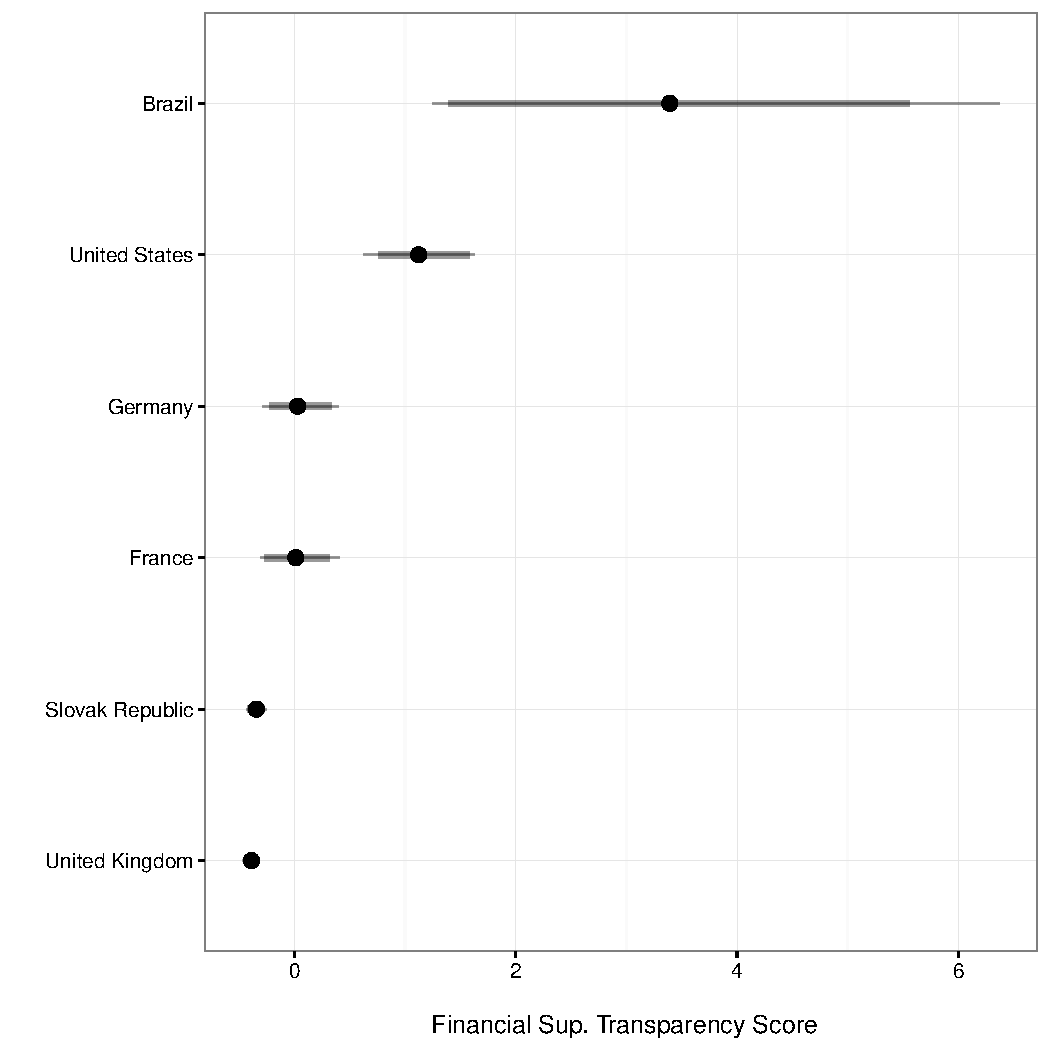
\includegraphics[scale=0.4]{figures/frt_uncertainty.pdf}
    \end{center}

}

\frame{
    \frametitle{In this course}

    In this course, we won't be covering more advanced ways to quantify your uncertainty about your composite indicators.

    \vspace{0.5cm}

    However, when you should be {\large{careful and honest when you compare units by ranking}} their composite scores.

    \vspace{0.5cm}

    {\large{Be honest about what you don't know.}}

}

\frame{
    \frametitle{Pros and Cons of Composite Indicators}

    \begin{table}
        {\footnotesize{
        \begin{tabular}{p{4cm} p{4cm}}
            Pros & Cons \\
            \hline\hline \\[0.1cm]
            Summarise complex multi-dimensional concepts & May be misleading if poorly constructed/non-transparent/interpreted \\[0.1cm]
            Support policy-making & May lead to simplistic policy conclusions or missed to support particular predefined policy goal \\[0.1cm]
            Facilitate communication with the public. & May disguise problems in one dimension if construction is not transparent. \\[0.1cm]
             & May exaggerate differences between units if uncertainty is not acknowledged.\\[0.1cm]

            \hline
        \end{tabular}
        }}
    \end{table}

    Partially from OECD (2008)

}

\end{document}
